\section{模型二：关键语音生物标志物识别}

\subsection{输入、方法与输出}

模型二使用 Dataset 1 subject-level 数据，共 252 名受试者，其中 Healthy 64 名、PD 188 名。输入特征为 752 个声学特征，排除 \feature{id}、\feature{gender}、\feature{class} 和 \feature{sex_male}。候选特征识别方法包括 Mann-Whitney U 检验、Welch t-test、FDR-BH 多重检验校正、Cohen's \(d\)、Cliff's delta、L1 Logistic 稳定选择、ExtraTrees 重要性和 held-out permutation importance。最终排序综合单变量差异、效应量、稳定性和模型重要性，而不是依赖单一树模型重要性。

\subsection{Top20 候选语音生物标志物}

\begin{longtable}{cllc}
\caption{Dataset 1 Top20 候选语音生物标志物}\label{tab:top20}\\
\toprule
序号 & 特征 & 类别 & Mean Rank \\
\midrule
\endfirsthead
\toprule
序号 & 特征 & 类别 & Mean Rank \\
\midrule
\endhead
1 & \feature{std_delta_delta_log_energy} & Delta / Delta-delta & 5.6667 \\
2 & \feature{std_6th_delta_delta} & Delta / Delta-delta & 15.5000 \\
3 & \feature{std_8th_delta} & Delta / Delta-delta & 20.6667 \\
4 & \feature{std_9th_delta_delta} & Delta / Delta-delta & 70.5833 \\
5 & \feature{std_7th_delta_delta} & Delta / Delta-delta & 79.4167 \\
6 & \feature{tqwt_TKEO_std_dec_12} & TQWT & 80.8333 \\
7 & \feature{tqwt_minValue_dec_12} & TQWT & 85.0000 \\
8 & \feature{std_9th_delta} & Delta / Delta-delta & 85.6667 \\
9 & \feature{mean_MFCC_2nd_coef} & MFCC & 86.1667 \\
10 & \feature{tqwt_TKEO_std_dec_11} & TQWT & 95.0833 \\
11 & \feature{std_10th_delta} & Delta / Delta-delta & 96.0833 \\
12 & \feature{tqwt_maxValue_dec_11} & TQWT & 97.4167 \\
13 & \feature{std_7th_delta} & Delta / Delta-delta & 97.6667 \\
14 & \feature{tqwt_kurtosisValue_dec_36} & TQWT & 101.5000 \\
15 & \feature{std_6th_delta} & Delta / Delta-delta & 101.9167 \\
16 & \feature{tqwt_kurtosisValue_dec_27} & TQWT & 103.7500 \\
17 & \feature{tqwt_energy_dec_12} & TQWT & 112.5833 \\
18 & \feature{DFA} & Nonlinear & 118.4167 \\
19 & \feature{tqwt_entropy_shannon_dec_17} & TQWT & 128.0833 \\
20 & \feature{tqwt_stdValue_dec_7} & TQWT & 131.6667 \\
\bottomrule
\end{longtable}

\subsection{结果解释}

Top20 中 Delta / Delta-delta 动态谱波动特征和 TQWT 多尺度特征占主要部分。Top50 类别分布为：TQWT 31 个，Delta / Delta-delta 16 个，Shimmer 1 个，MFCC 1 个，Nonlinear 1 个。该分布提示 PD/Healthy 的声学差异主要体现在动态谱波动和多尺度时频结构上。

\begin{figure}[H]
\centering
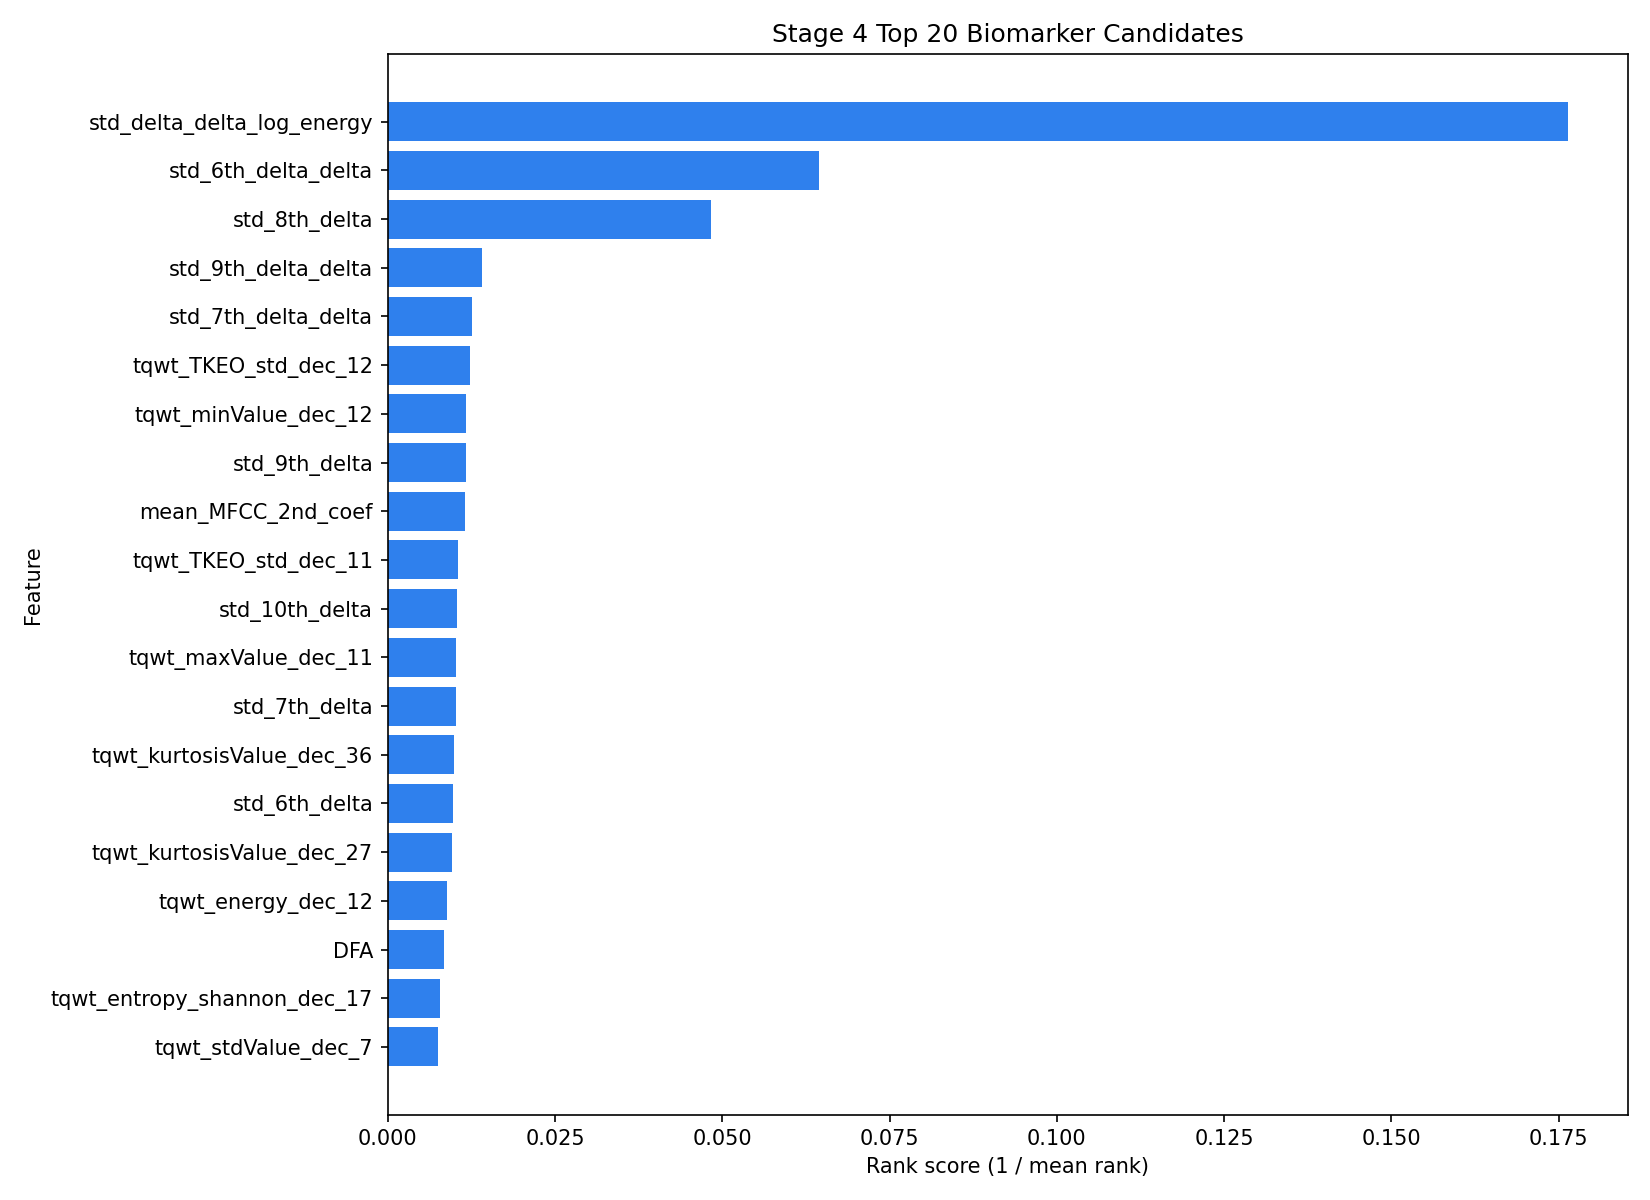
\includegraphics[width=0.86\textwidth]{figures/stage4_top20_biomarker_rank.png}
\caption{Top20 候选语音生物标志物综合排序}
\end{figure}

\begin{figure}[H]
\centering
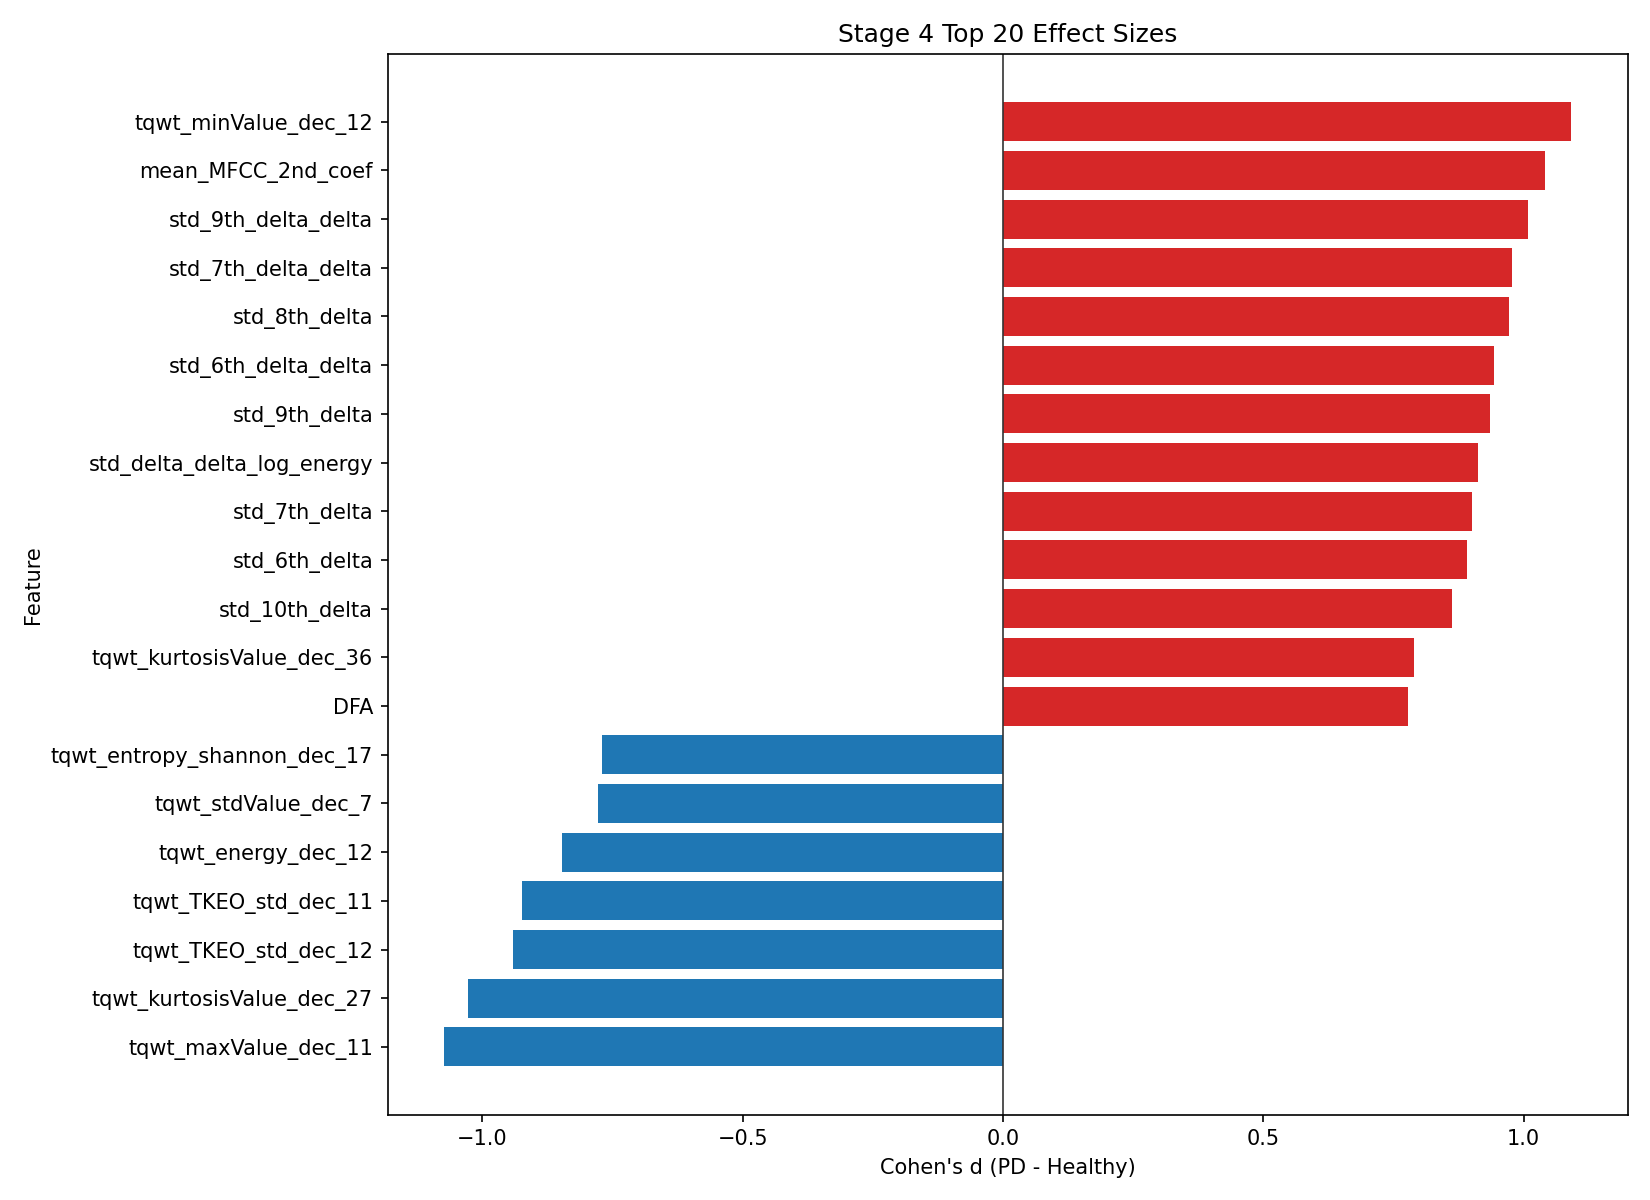
\includegraphics[width=0.86\textwidth]{figures/stage4_top20_effect_size.png}
\caption{Top20 候选特征效应量}
\end{figure}

\begin{figure}[H]
\centering
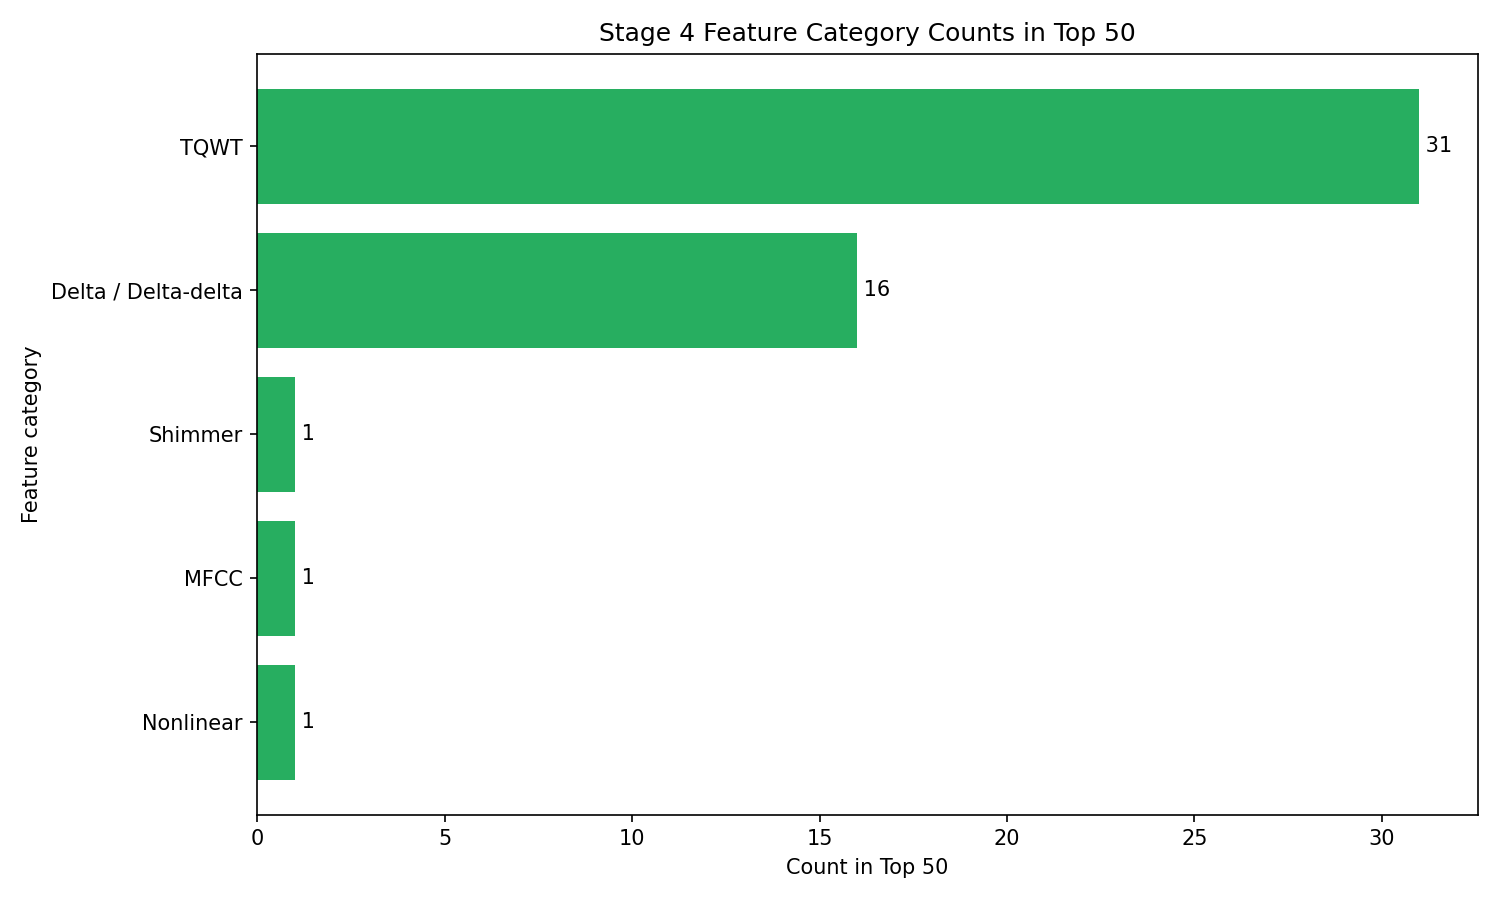
\includegraphics[width=0.72\textwidth]{figures/stage4_feature_category_counts_top50.png}
\caption{Top50 候选特征类别分布}
\end{figure}

上述特征只能称为候选语音生物标志物或判别性声学特征。由于本文没有临床机制实验和外部因果验证，不能作因果机制外推。
